\section{Forschungsplann}

Die Literatur bezüglich Netzwerksicherheit, bargeldlose Zahlungsverfahren und Vending Machines ist 
in den letzten 20 Jahren deutlich umfangreicher geworden. Da diese Begriffe viele und fast unendliche 
Konzepte decken, gehen wir hier auf spezifische Aspekte dieser Begriffe ein und zwar 
auf die Sicherheit von drahtlosen Zahlungsmethode und von Smartcards. Folgende Quelle tragen zu der
Suchen nach vertrauenswürdigen Informationen bei:

\begin{itemize}
    \item ScienceDirect;
    \item Researchg Gate;
    \item IEEE Xplore;
    \item Google Scholar.
\end{itemize}

Die Recherche fasst sich hauptsächlich in der Sammlung aus dem spezialisierten Literatur von Konzepten,
Sicherheitslücken und Gegenmaßnahmen von den oben genannten Elementen zusammen:

\vfill
\begin{figure}[htb]
    \centering{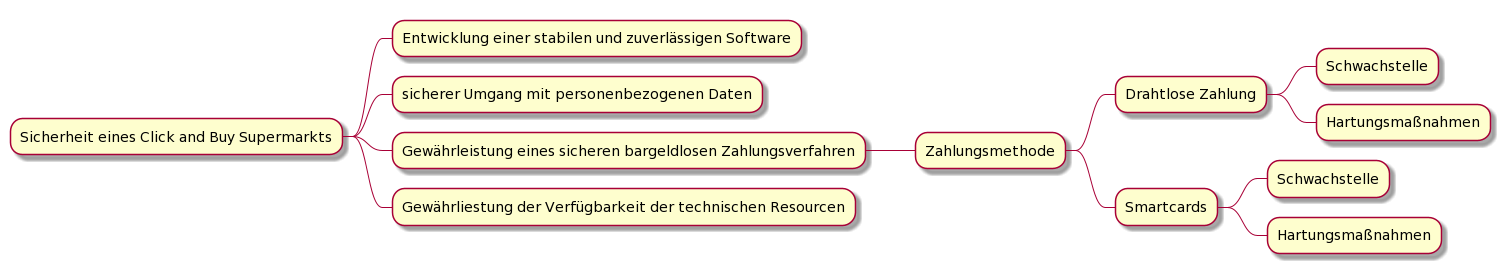
\includegraphics[width=12cm]{Bilder/Diagram2.png}}
    \caption{Recherchespfad (eigenes Bild)}
    \label{fig:diagramrecherche}
\end{figure}
\vfill
